\documentclass{suturo}
\usepackage{spverbatim}

\begin{document}
    \maketitle{Knowledge}{05.01.2018}{}{1}{}{}{}{}

\makeatletter
\newcommand{\chapterauthor}[1]{%
  {\parindent0pt\vspace*{-47pt}%
  \linespread{2.2}\large\begin{flushright}von: #1\end{flushright}%
  \par\nobreak\vspace*{0pt}}
  \@afterheading%
}
\makeatother

\section{Architektur und Funktion}
\subsection{knowledge\_grasp}
\chapterauthor{Max-Phillip Bahr}
Das Knowledge\_Grasp-Paket dient dazu die GraspPose zu einem erkannten Gegenstand aus der Ontologie auszulesen, an der der PR2 diesen Gegenstand vor ihm greifen soll.

\begin{figure}[!htb]
        \center{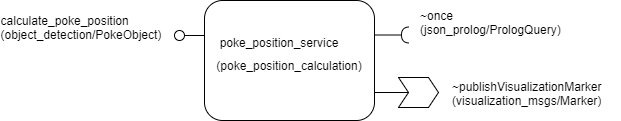
\includegraphics[width=\textwidth]
        {figures/pokepositionnode.png}
        \caption{\label{fig:poke_position_service_node} Architektur der knowledge\_grasp\_service-node}}
\end{figure}
      
\section{Methodenbeschreibung}
\subsection{knowledge\_grasp}
\chapterauthor{Max-Phillip Bahr}

\subsubsection{find\_grasp\_pose - Prolog}
\begin{spverbatim}
find_grasp_pose(ObjectClassLabel, Position, Quaternion)
@param ObjectClassLabel Das Objektlabel des zu greifenden Objekts 
       (z.B. suturo_object:'JaMilch')
@param Position Position der GraspPose als Prolog Liste (z.B. [0.0, 0.0, 0.0])
@param Quaternion Orientation der GraspPose also Prolog Liste 
       (z.B. [0.0 0.0 0.0 1.0])

Description : Liest zu einem gegebenen Objektlabel eine zugehörige GraspPose aus der Ontologie aus. Es wird bei der eingespeicherten GraspPose von der Translation des Grippers zum Mittelpunkt des Objekts ausgegangen.
\end{spverbatim}

\subsubsection{createQuery - C++}
\begin{spverbatim}
std::string createQuery(std::string object_label)
@param object_label Das Objektlabel.
@return Den aus dem Objektlabel zusammengesetzten Query-String.

Description : Baut aus dem Objektlabel einen Query-String für die Prolog-Methode find_grasp_pose zusammen.
\end{spverbatim}

\subsubsection{find\_grasp\_pose - C++}
\begin{spverbatim}
bool find_grasp_pose(knowledge_msgs::GraspIndividual::Request  &req, 
                             knowledge_msgs::GraspIndividual::Response &res)
@param req Adresse des Request Objekts von GraspIndividual das bearbeitet werden soll.
@param res Adresse zum schreiben des Response Objekts von GraspIndividual.
@return true wenn Methode erfolgreich, false wenn nicht.

Description : Die Methode liest das Objektlabel aus req aus und baut mit createQuery einen QueryString  der mit der once-Methode an den Prolog Server geschickt wird. Wenn Prolog mit find_grasp_pose (Prolog Methode) eine Lösung zur Query findet (also die GraspPose aus der Ontologie ausliest) wird diese in das Response Objekt 
geschrieben und true zurückgegeben. Wenn nicht wird eine Fehlermeldung ausgegeben und false zurückgegeben.
\end{spverbatim}



\section{Schnittstellen}
\chapterauthor{Max-Phillip Bahr}

\subsection{Service Server knowledge\_grasp\_service/knowledge\_grasp}
\begin{spverbatim}
GraspIndividual.srv
@request:

	string object_label

@response: 

	geometry_msgs/PoseStamped grasp_pose
\end{spverbatim}
Wir entnehmen der Message das Objektlabel und lesen die für dieses Objekt gespeicherte GraspPose aus der Ontologie aus. Die Pose wird als grasp\_pose zurückgegeben.

\section{Programmablauf}
\subsection{knowledge\_grasp}
\begin{itemize}
\item[1.]Es wird eine Anfrage an den Service-Server gestellt
\item[2.]Eine Anfrage mit folgendem Inhalt wird an den json\_prolog- Server wird gestellt:\\ "find\_grasp\_pose(suturo\_object:'object\_label', Position, Quaternion)." 
\item[3.]Die entsprechende Prolog Methode liest die zum übergebenen Objektlabel gehörige GraspPose aus der OWL Ontologie aus.
\item[4.] Die als PrologBindings vom json\_prolog- Server erhaltene GraspPose wird von find\_grasp\_pose (c++) in die gewünschte Form konvertiert.
\item[5.] Antwort zurückgeben.
\end{itemize}

\end{document}
